\section{Langkah-Langkah Percobaan}
$\bullet$ Wireless Point-to-Point
\begin{enumerate}
	\item Reset Router untuk memastikan tidak ada sisa konfigurasi dari praktikum sebelunya
	\item Log in ke Router
	\item Atur Router A sebagai Bridge melalui interface Wireless -> wifi interface. Dan berikan nama PointToPoint\_2\\
	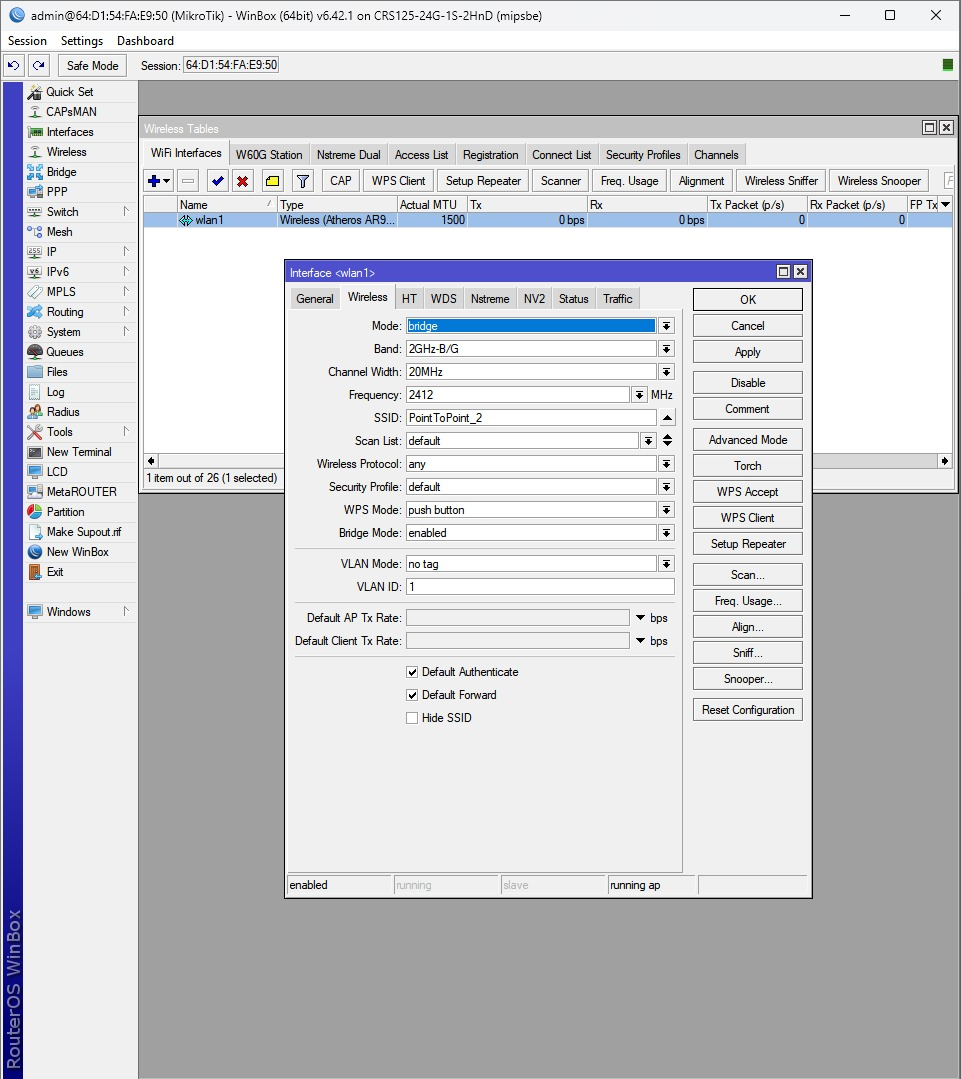
\includegraphics[width=0.5\textwidth]{p4/img/bridge.jpg}
	\item Atur Router B sebagai Station
	\item Pada Router B, klik scan, kemudian cari nama "PointToPoint\_2" dan klik connect
	\item Atur IP WLAN pada router A sebagai 10.10.10.1/29 dengan interface WLAN1
	\item Atur IP WLAN pada router B sebagai 10.10.10.2/29 dengan interface WLAN1
	\item Atur IP router pada router A sebagai 192.168.20.1/24 dengan interface ether1
	\item Atur IP router pada router B sebagai 192.168.30.1/24 dengan interface ether1
	\item Atur IP laptop yang terhubung pada router A sebagai 192.168.20.2/24
	\item Atur IP laptop yang terhubung pada router A sebagai 192.168.30.2/24
	\item Tambahkan alamat untuk Routing pada menu routing -> address\\
	\item Tambahkan alamat IP network (192.168.xx.0) ke routing\\
	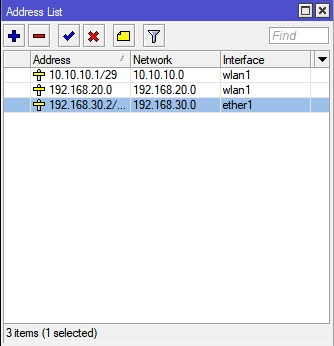
\includegraphics[width=0.5\textwidth]{p4/img/address.jpg}
	\item Uji ping antar router\\
	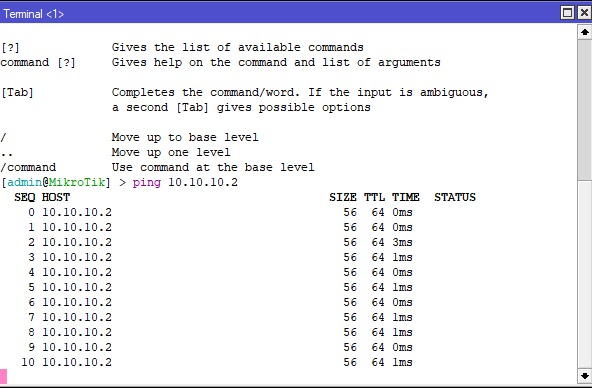
\includegraphics[width=0.4\textwidth]{p4/img/pingrslt3.jpg}
	\item uji ping antar PC\\
	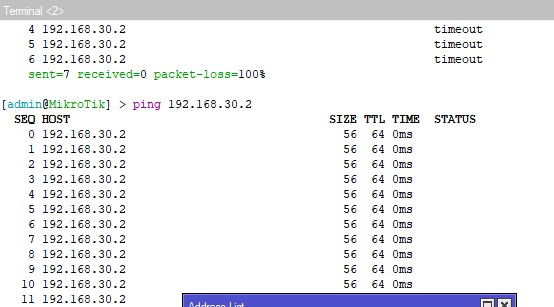
\includegraphics{p4/img/pingrslt2.jpg}
\end{enumerate}
$\bullet$ Wireless Point-to-Multipoint
\begin{enumerate}
	\item Reset Router untuk memastikan tidak ada sisa konfigurasi dari praktikum sebelunya
	\item Log in ke Router
	\item Atur Router A sebagai Ap Bridge melalui interface Wireless -> wifi interface. Dan berikan nama PointToPoint\_2\\
	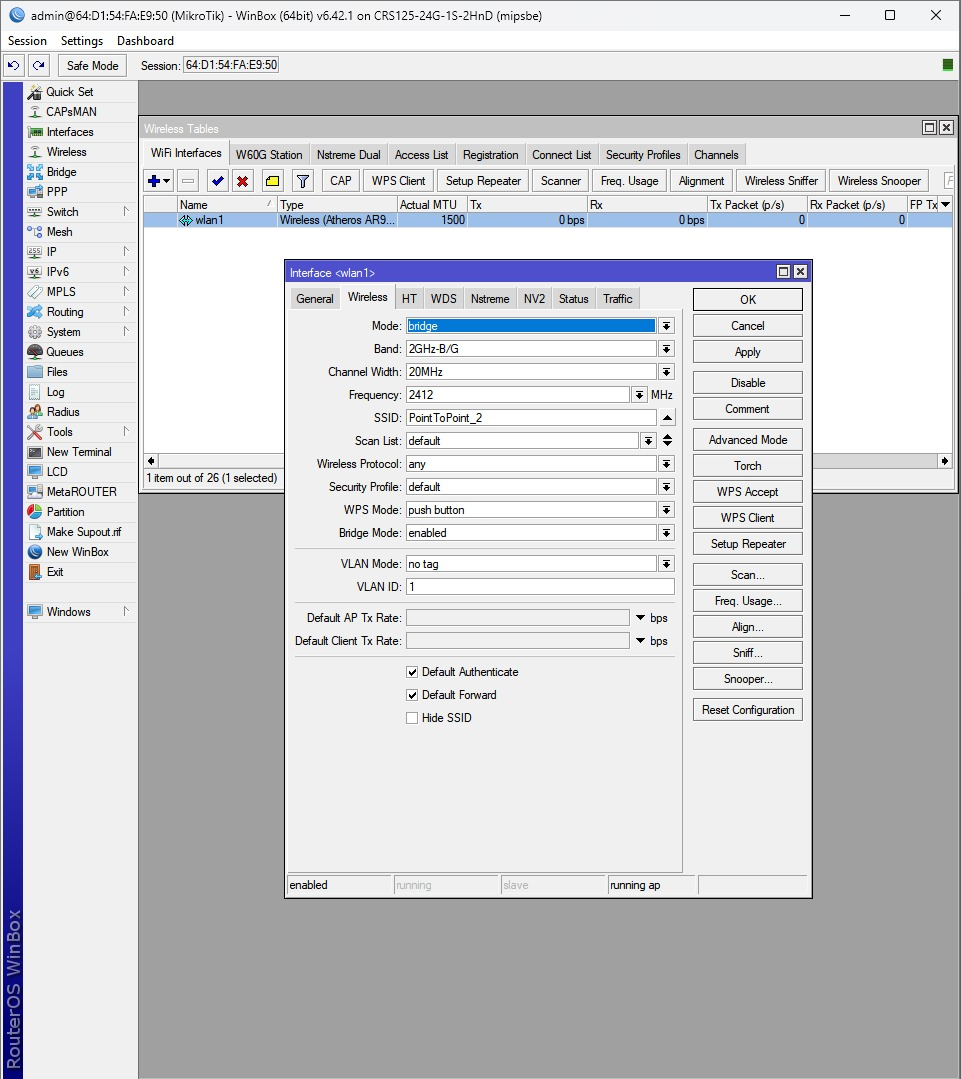
\includegraphics[width=0.5\textwidth]{p4/img/bridge.jpg}
	\item Atur Router B sebagai Station
	\item Pada Router B, klik scan, kemudian cari nama "PointToPoint\_2" dan klik connect, setelah connect maka station akan berubah menjadi AP station
	\item Atur IP WLAN pada router A sebagai 10.10.10.1/29 dengan interface WLAN1
	\item Atur IP WLAN pada router B sebagai 10.10.10.2/29 dengan interface WLAN1
	\item Atur IP router pada router A sebagai 192.168.20.1/24 dengan interface ether1
	\item Atur IP router pada router B sebagai 192.168.30.1/24 dengan interface ether1
	\item Atur IP laptop yang terhubung pada router A sebagai 192.168.20.2/24
	\item Atur IP laptop yang terhubung pada router A sebagai 192.168.30.2/24
	\item Tambahkan alamat untuk Routing pada menu routing -> address\\
	\item Tambahkan alamat IP network (192.168.xx.0) ke routing\\
	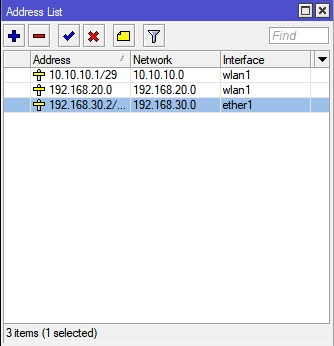
\includegraphics[width=0.5\textwidth]{p4/img/address.jpg}
	\item Uji ping antar router\\
	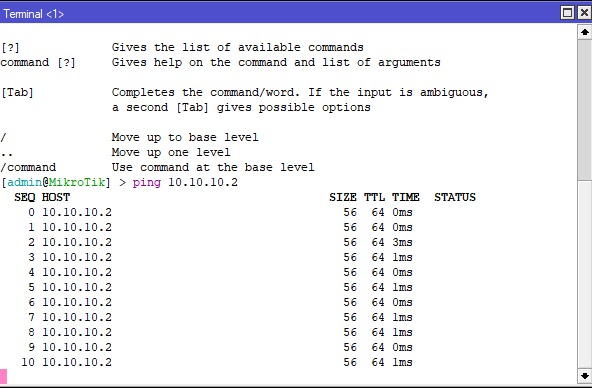
\includegraphics[width=0.4\textwidth]{p4/img/pingrslt3.jpg}
	\item uji ping antar PC\\
	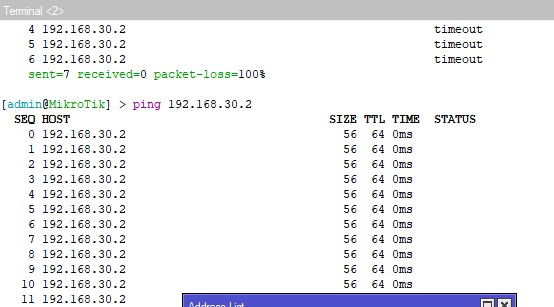
\includegraphics{p4/img/pingrslt2.jpg}
\end{enumerate}
$\bullet$ Wireless Bridge
\begin{enumerate}
	\item Reset Router untuk memastikan tidak ada sisa konfigurasi dari praktikum sebelunya
	\item Log in ke Router
	\item Atur Router A sebagai Bridge melalui interface Wireless -> wifi interface. Dan berikan nama PointToPoint\_2\\
	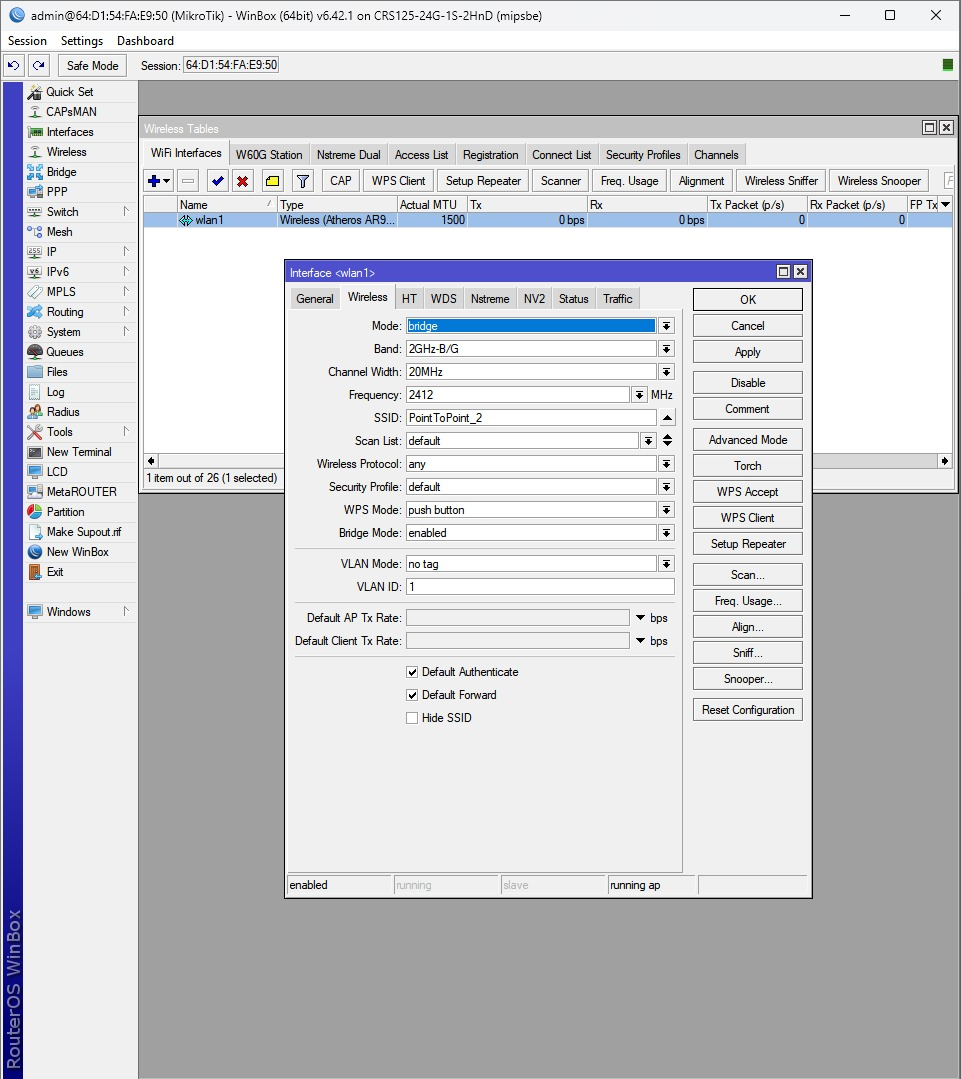
\includegraphics[width=0.5\textwidth]{p4/img/bridge.jpg}
	\item Atur Router B sebagai Station pseudobridge
	\item Pada Router B, klik scan, kemudian cari nama "PointToPoint\_2" dan klik connect
	\item Atur IP WLAN pada router A sebagai 10.10.10.1/29 dengan interface WLAN1
	\item Atur IP WLAN pada router B sebagai 10.10.10.2/29 dengan interface WLAN1
	\item Atur IP router pada router A sebagai 192.168.20.1/24 dengan interface ether1
	\item Atur IP router pada router B sebagai 192.168.30.1/24 dengan interface ether1
	\item Atur IP laptop yang terhubung pada router A sebagai 192.168.20.2/24
	\item Atur IP laptop yang terhubung pada router A sebagai 192.168.30.2/24
	\item Tambahkan alamat untuk Routing pada menu routing -> address\\
	\item Tambahkan alamat IP network (192.168.xx.0) ke routing\\
	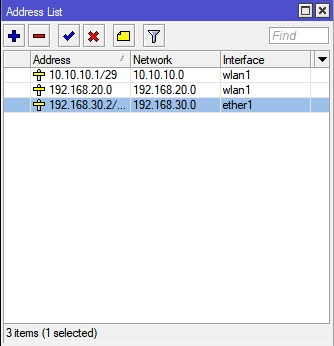
\includegraphics[width=0.5\textwidth]{p4/img/address.jpg}
	\item Uji ping antar router\\
	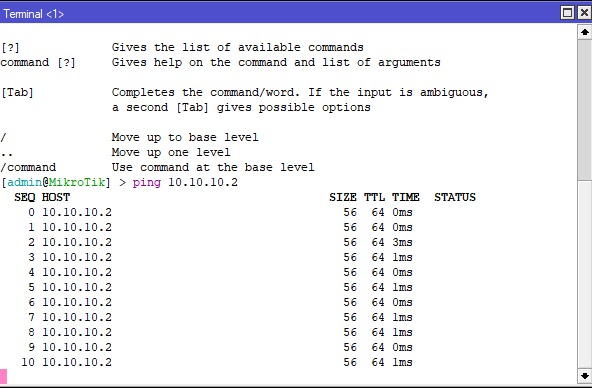
\includegraphics[width=0.4\textwidth]{p4/img/pingrslt3.jpg}
	\item uji ping antar PC\\
	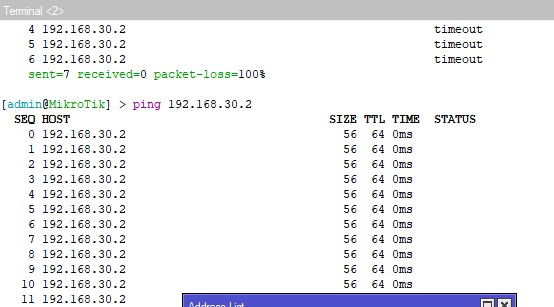
\includegraphics{p4/img/pingrslt2.jpg}
\end{enumerate}
\section{Analisis Hasil Percobaan}
Dari percobaan yang dilakukan terdapat 3 percobaan\\
$\bullet$ Point-to-Point\\
Dari percobaan yang dilakukan dimana satu Router diatur sebagai bridge, dan satu router diatur sebagai station. Ketika dicoba dilakukan ping antar Router telah berhasil. Artinya routing wireless point-to-point telah berhasil dilakukan\\
$\bullet$ Point-to-Multipoint\\
Dari percobaan yang dilakukan dimana satu Router diatur sebagai Ap bridge dan satu router diatur sebagai AP station. Seharusnya Router AP bridge dapat dihubungkan ke beberapa device secara langsung karena itu disebut Multipoint. Namun karena hanya terdapat 1 PC yang terhubung tidak dapat diuji fungsi Multipoint ini. Ketika dilakukan uji ping antar Router, didapatkan hasil berhasil. Artinya routing wireless point-to-multipoint telah berhasil dilakukan\\
$\bullet$ Wireless Bridge\\
Dari percobaan yang dilakukan dimana satu Router diatur sebagai Bridge dan satu router diatur sebagai Station pseudobridge. Setting ini seharusnya menghasilkan sebuah bridge yang memungkinkan dua jaringan LAN untuk saling bertukar informasi. Namun tidak dilakukan pengujian untuk hal ini. Ketika dilakukan uji ping antar router, didapatkan hasil berhasil. Artinya routing wireless bridge telah berhasil dilakukan

\section{Hasil Tugas Modul}
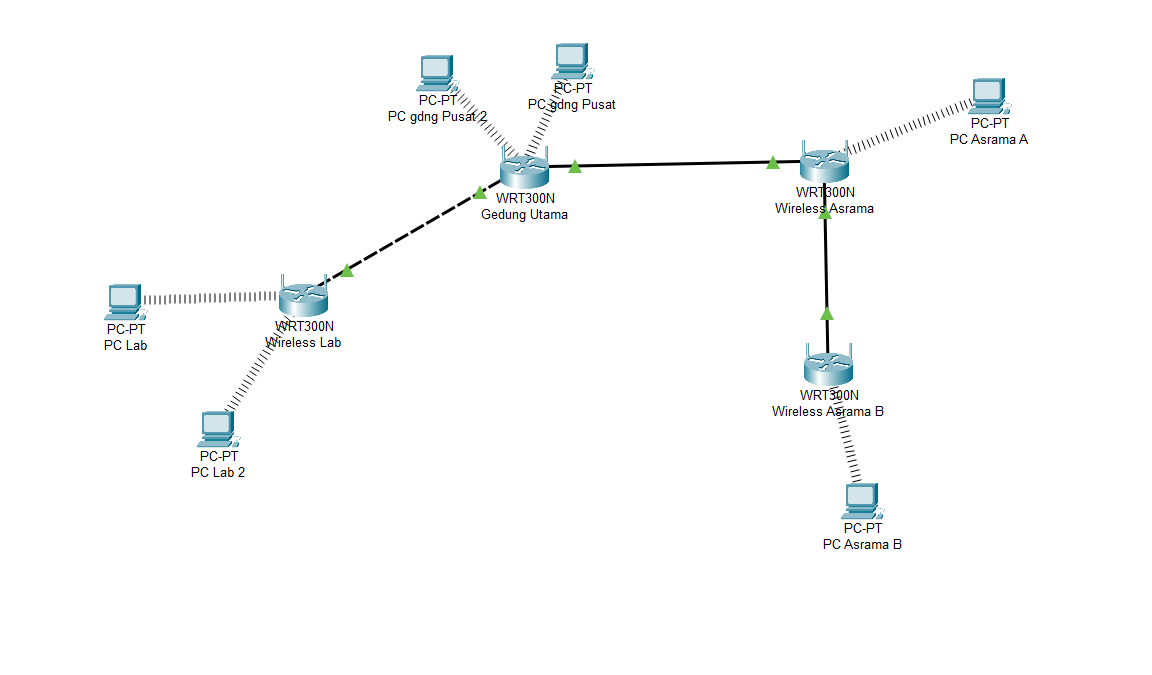
\includegraphics[width=0.7\textwidth]{p4/img/tumod.png}\\
Dari hasil Topologi diatas, dapat dilakukan ping Antar PC di satu gedung yang sama, dan PC\\
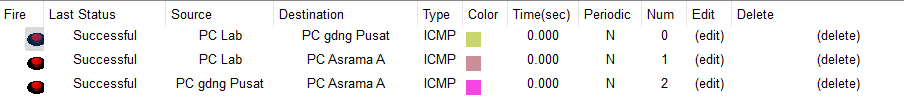
\includegraphics[width=1.0\textwidth]{p4/img/tumod2.png}\\
Digunakan penghubungan dengan kabel antar router di setiap gedung karena praktikan tidak dapat melakukan penghubungan antar router secara wireless dan praktikan tidak menemukan tutorial yang memberikan cara menghubungkan antar router secara wireless

\section{Kesimpulan}
Dari praktikum yang telah dilakukan, dapat disimpulkan bahwa penghubungan secara wireless dapat dilakukan dalam beberapa mode yang memiliki fungsi yang berbeda. Seperti Point-to-Point yang menghubungkan secara langsung antara 2 perangkat, Point-to-Multipoint yang menghubungkan beberapa perangkat ke satu perangkat, dan wireless bridge yang menghubungkan antar 2 LAN. Kemudian dari praktikum juga dapat disimpulkan bahwa set up untuk routing wireless lebih sederhana dibandingkan wired.

\section{Lampiran}
\subsection{Dokumentasi saat praktikum}
Hasil beberapa tes ping yang dicoba\\
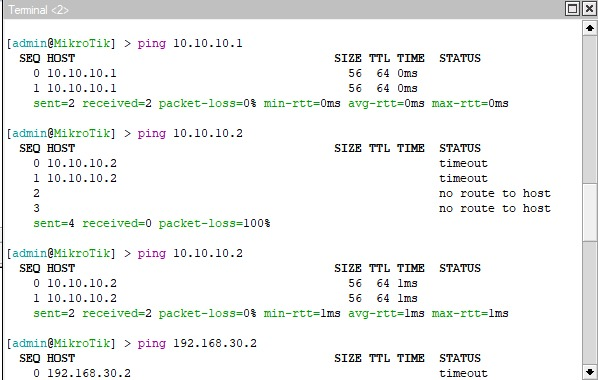
\includegraphics{p4/img/pingrslt1.jpg}

